\documentclass[10pt,a4paper]{article}
\usepackage[utf8]{inputenc}
\usepackage{amsmath}
\usepackage{amsfonts}
\usepackage{amssymb}
\usepackage{graphicx}
\usepackage{framed}
\usepackage{float}
\usepackage{array}
\usepackage{adjustbox}
\usepackage[normalem]{ulem}
\useunder{\uline}{\ul}{}
\usepackage{hyperref}
\author{Paul Cowie \and Jacob Ford \and Nicole Munro \and William Kavanagh \and Ben Procter \and Pregashni Mohanarajah }
\date{}
\title{Team Six: IS(H) AX2, Final Report}
\begin{document}
\maketitle

\section*{City Council Briefing}

Our application, 120 Degrees, offers users an experience unmatched by any other currently available. Through the use of multidimensional query functionality, our application allows users to rank restaurants in their vicinity based on multiple terms simultaneously. The power of our application comes from the basic yet functional interaction of the user generating results highly specific to their needs. This advanced functionality is all provided within a polished, professional product that is pleasing to the eye designed without superfluous visual flair obstructing user-interaction.

The main element of our product that makes us stand out is how we deal with user search querying. By allowing multiple, weighted queries that can be deemed either positive or negative, we can immediately deliver more precise suggestions than competitors. There are not many other services which allow users to negatively mark certain aspects of a restaurant in the way our website does and this allows us to remove several suggestions in which the user would have no interest. We believe that what users specifically do not want is as important as what they do. In an ever-growing and highly competitive market such as the world of food, sifting through the vast quantity of offers efficiently can only be done if users can specify the negative attributes that they find undesirable alongside what is important to them. Searching for everything simultaneously also makes our service significantly more efficient for our users relative to other services, and all without sacrificing any of the functionality offered by our competitors. Speed and efficiency are two metrics which have become even more important than they were before in the current climate in which the everyday consumer is more tech-savvy than ever. The ranking of queries is also a feature unique to 120 degrees that results in users getting personalised results. The services currently available will allow for searching by a single cuisine, whereas with 120 degrees users can search for multiple at a time and rank them by preference. “I really want Indian, but I wouldn’t mind getting pizza” - this form of query is possible with 120 degrees in a single search, functionality that is not offered by any services currently on the market. Through our unique approach to searching users will get a service that is more efficient, more personalised and more accurate than the currently available applications offering similar services.

Another element of our design which allows for users to obtain suggestions more highly tuned to their specifics needs is the ability to search for literally any term they can think of - There are not many other services which allow users to search for how “swanky” or “ambient” a restraunt is. This is another example of unique functionality that our application provides whilst also keeping an intuitive design that all users will be able to understand in mere moments. In designing the application we wanted to ensure we catered to every need and from a discussion on this topic we had the idea to allow users to search for absolutely everything, thereby ensuring all of their needs were addressed. This functionality also means that although we designed our product with several key user groups in mind, our website caters to everyone. Paired with an attractive but understated visual design, this functionality ensures no-one will feel that they are not the intended audience for the product.

We worked very hard when building this product to ensure that functionality was not sacrificed for simplicity and vice-versa. This endeavour has left us with a product that is as easy to use as any currently available, but one that we believe will generate more specific results than any other. The way in which our results are displayed was designed to best incorporate the associative ranking we give each restaurant, whilst also being both attractive and iconic, a way to visually set our product apart from others. This distinctiveness is something we strongly believe we have achieved by displaying our results as tessellating hexagons which can be highlighted to give interaction options for a restaurant and which is coloured to distinguish the correlation to the user’s multidimensional query.

Our product offers all of the key elements offered by similar applications, whilst also expanding on them to give users more control of the suggestions that are generated. It uses user’s location data to search by distance, and it allows for searching by cuisine, price and average rating - but for the first time, users can search by these criteria concurrently. This functionality allows for a much more streamlined process. All of this, in addition to being able to search for custom queries and assigning weight to any given query, delivered in a professional and intuitive environment, puts our product to the forefront of the food-finding field. 

\section*{Design Requirements}

From the original concept, we set out with the aim of designing an interface that would allow users to search various ‘keywords’ allowing them to choose the categories that they have the highest/lowest preference to. 

\begin{figure}[H]
	\begin{center}
		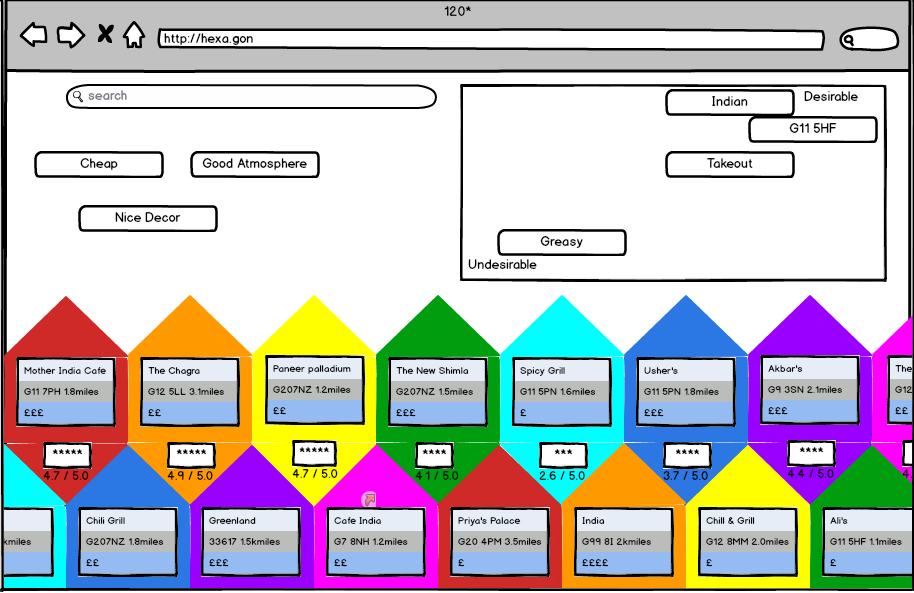
\includegraphics[scale=0.37]{Screenshot.png}
		\caption{Paper prototype of design}
		\label{figure:prototype}
	\end{center}
\end{figure}


We were able to achieve this through its incorporation into the pinboard system where choices were split between cuisine types and other metrics such as ‘Nut-Free’ or ‘Expensive’. We also allowed the users the create their own if there were options that had not been taken into consideration.

\begin{figure}[H]
	\begin{center}
		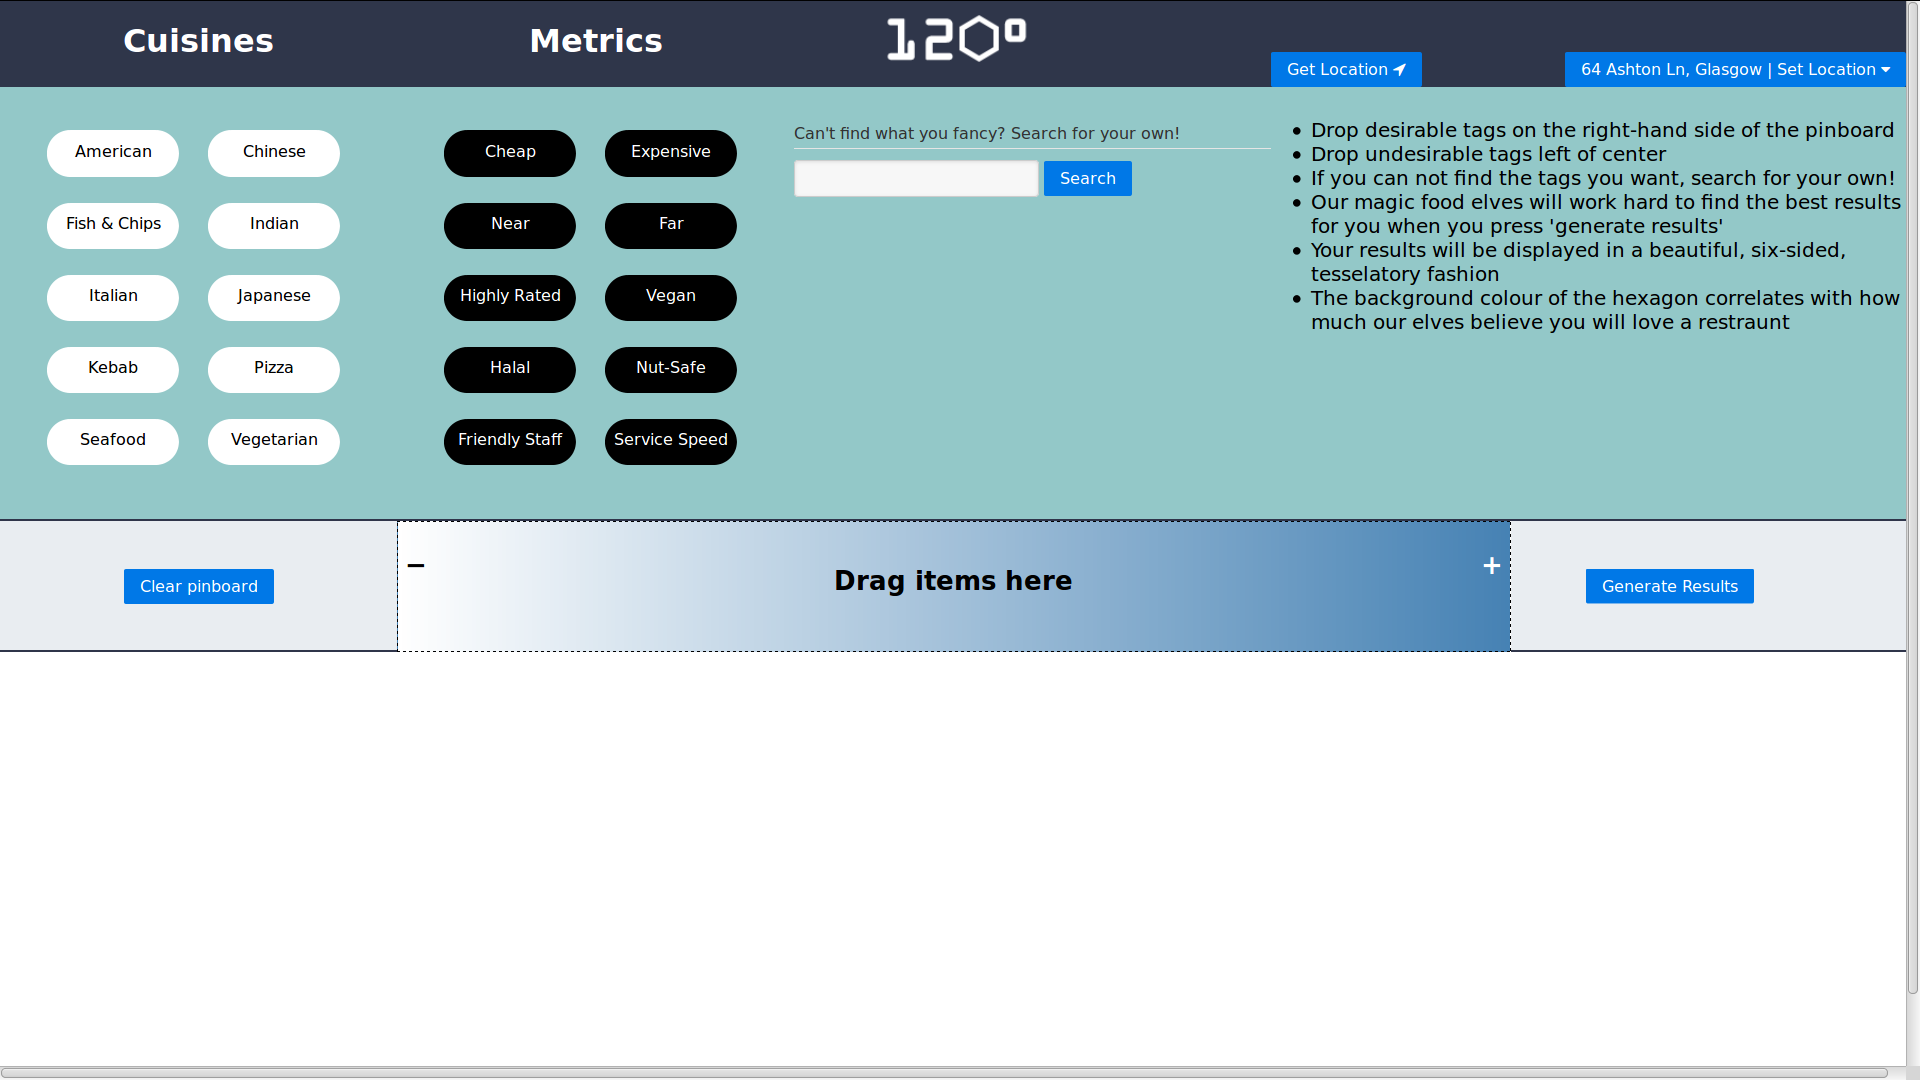
\includegraphics[scale=0.2]{newScreenshot.png}
		\caption{Finished design without results}
		\label{figure:finished-design-no-results}
	\end{center}
\end{figure}

\begin{figure}[H]
	\begin{center}
		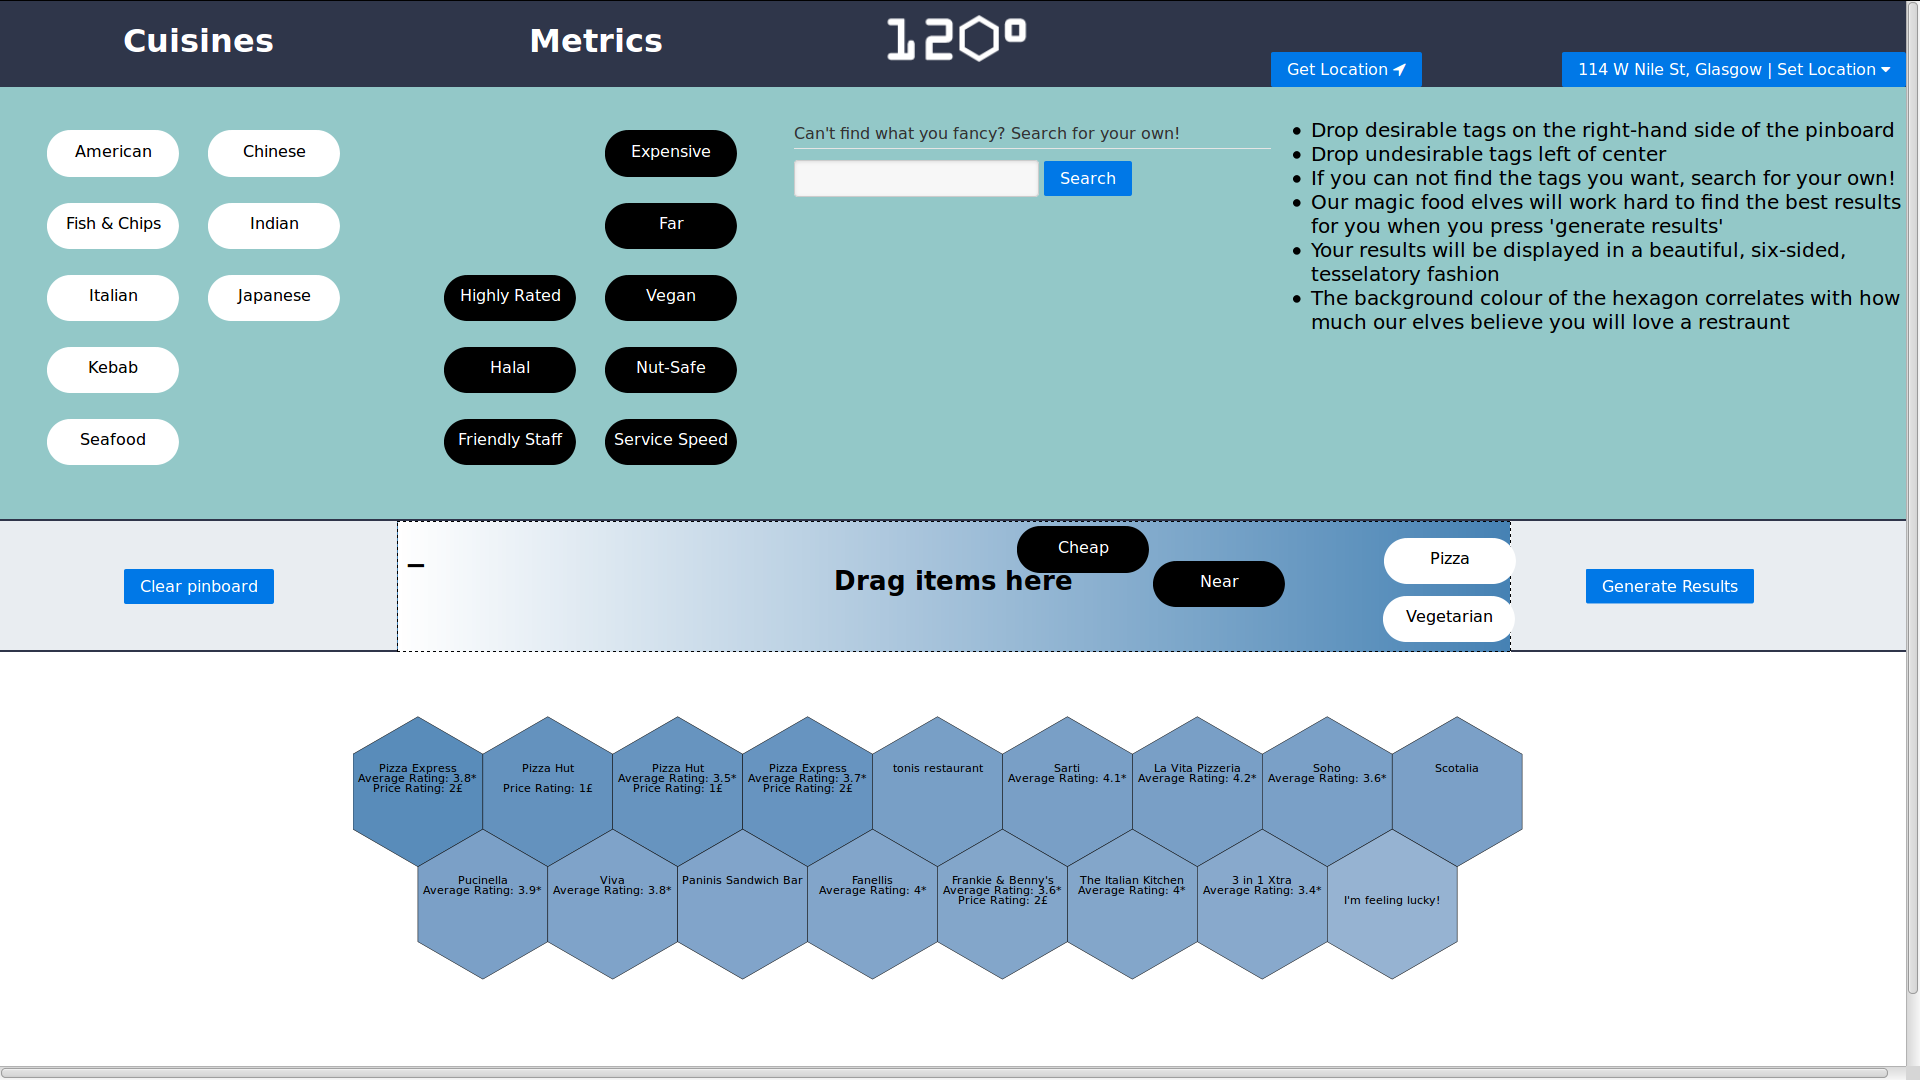
\includegraphics[scale=0.2]{newScreenshotWithResults.png}
		\caption{Finished design with results}
		\label{figure:finished-design-with-results}
	\end{center}
\end{figure}

One of the key features of our design was that the results were to be displayed in an iconic hexagonal design. Originally, the plan was to have the hexagons tessellating across the screen in a variety of different colours. However, as the design process went on, we made the team decision that it would make more sense to have a gradient colour scheme which gets paler the worse the result matched the query. This can be seen in Figure \ref{figure:finished-design-with-results} where the hexagons, starting on the top left and finishing at the right of the bottom row, gradually fade from steel blue to a paler shade. We also changed the original design for inspecting hexagons from expanding to highlighting, to better utilize the space available both within the hexagon and around it.

In the original concept, the pinboard was to have the design running from bottom left to top right representing the least desirable to the most respectively. However, due to time constraints and also to make better use of the whole screen, we decided that it would make more sense to make the pinboard operate purely on a 2-D Axis where preference towards certain tags was determined by its location on the x-axis with preference increasing the further to the right of the axis a tag was placed by the user.

The decision was also taken to move the pinboard from the top of the screen to the centre. This was due to its ability to created a divider between the searching components at the top of the page and the hexagonal results that are generated and displayed below.

\section*{Submission Description}

Many of the original design decisions carried through to the final product. Our key features - the multitude of tags, the highly interactive pinboard, and the use of hexagons to display results - are all present in the final product. They have all experienced minor changes to better suit the formatting of the website and the data - the pinboard is now completely horizontal and resides in the middle of the screen, while the search bar and suggested tags occupy the top third. The hexagons also display slightly different data based on the results returned by the Google Places API, and highlight rather than expand when clicked. The multi-dimensional search algorithm was largely implemented as envisioned, but some Google Places API limitations prevented the idea to be explored in full. We also included several new features, including a map for the user to choose their location and tips for effective use, as much of the functionality is not immediately apparent upon first visiting the site. We also decided to introduce an “I’m feeling lucky” mystery hexagon, for a bit of fun in our design.

However, several bits of functionality were ultimately not included. One feature that did not make it to the final product was the idea that the hexagons would update as the user dragged tags to the pinboard. This was discarded due to the complexity of the algorithm and the amount of data being sent to and returned from the Google Places API to generate the best results possible. In addition, due to the required queries, fewer results are displayed than originally intended, with many being truncated by the limit on the number of queries one webpage can request of Google. We decided to keep the result count low to allow for higher-quality results that best match the search terms.

\section*{Analytical Findings}

It is vital to test a system on actual users between design iterations. During the short design lifecycle of our product we performed two small user tests to ensure that we were creating a system that delivered on all of the aspects that we had intended it to. Our first test was performed once we first had a usable build of the system to ensure that the final stages of the creation, which are usually taken up with small visual tweaks, were going to make our product better. We carried out the second batch of testing once we believed we had finished the design of our product. The intention behind the second test was to ensure that we had achieved all that we had set out to and, that we had improved on the user experience with the changes we had made since the first tests.

To ensure that our results were significant, we asked the same tasks of the users in both of our experimental designs. We gave them three tasks to perform that, between them, encompassed all of the key functionality of our application to make sure that we were confident with the performance of every aspect of our design. We wanted to obtain quantitative results to allow for precise comparison between the two sets of data, however we also wanted qualitative data so that we knew what areas our users felt worked best and what areas were least effective as well as any suggestions they had for improvement. To this end, we took three metrics from each of the three tests we had our users perform; time taken to generate input similar to the desired input, any comments the user had on specific sections of the design and a report of the user’s performance written by whoever carried out the tests which we did not show the user.

To ensure that the tags used matched real-world usage, some repeatable, representative tasks were devised. Test participants were given no further input than a short sentence intended to duplicate real world scenarios in which we envisage our application being used. The sentences we used to prompt our participants were:


\begin{itemize}
\item \textbf{Task 1:} “Please search for an Italian restaurant that is both cheap and nearby where we are now.”
\item \textbf{Task 2:} “Please change the location to your home address and find Chinese or Thai food, but not Japanese food, in the vicinity.”
\item \textbf{Task 3:} “You have friends over when someone suggests going to a restaurant, please find a restaurant that preferably is kosher, but is definitely not American.”
\end{itemize}

\noindent After the  test we asked users to comment on:

\begin{itemize}
	\item The overall design and aesthetic of the application.
	\item The custom tag generation and the map.
	\item The form in which results are displayed.
\end{itemize}

\noindent The results are shown in Table \ref{table:experiment-1}


\subsection*{Investigation 1}

\begin{itemize}
\item{User 1:
\begin{itemize}
\item{Task 1: 

Time taken: 21s

User 1 described the design as ‘interesting, neat, and professional’, though he found the pinboard suspicious, questioning how intuitive it is.
His performance was poor, and it took two attempts to generate the correct input.}
\item{Task 2:

Time taken: 51s

User 1 described the map and the action of dropping the pin to change location as ‘tricky and time-consuming’, suggesting it would be difficult for mobile users. 
He did not realise he could search for the ‘Thai’ tag, and spent some time questioning how to proceed.}
\item{Task 3:

Time taken: 13s

User 1 said the result generation was ‘unique and interesting’. It was clear from his speed and efficiency that he had quickly learned to use the system.}
\end{itemize}}

\item{User 2:
\begin{itemize}

\item{Task 1:

Time taken: 30s

User 2 commented that the design was ‘definitely cool’, however, he questioned how useful the ability to score tags negatively would prove. He also suggested to clarify the specification, perhaps moving it to the left side of the screen.
He read the specification then performed the task perfectly.}
\item{Task 2:

Time taken: 2m, 13s

User 2 found the custom searching cool, though the map was ‘unclear’.
He found the map extremely difficult to use, finding his location but not understanding the drag functionality needed to change the location.}
\item{Task 3:

Time taken: 10s

User 2 suggested changing some of the metrics offered and questioned how many users would find use in ranking ‘Service speed’ lowly.
The user was much quicker, understanding the system and using our functionality to generate the specific results.}

\end{itemize}}

\item{User 3:
\begin{itemize}

\item{Task 1:

Time taken: 1m, 21s

User 3 found that the system was not clearly explained or intuitive, and suggested making the functionality explanation stand out more.
His first search did not match the task, not understanding the pinboard.}
\item{Task 2:

Time taken: 1m, 5s

User 3 liked the tag creation functionality.
User 3 spent much time on the map, but found the ability to search for tags impressive and intuitive.}
\item{Task 3:

Time taken: 11s

User 3 commented that the highlight overlay was ‘odd’ and suggested making the hover effect fade more quickly.
He was clearly interested with the iconic visual design decisions, however, questioned whether or not it was too bold.}

\end{itemize}}
\end{itemize}


\begin{table}[H]
\centering
\begin{tabular}{c|ccc|}
\cline{2-4}
                             &                             & Time Taken (s)                &        \\ \cline{2-4} 
                             & \multicolumn{1}{c|}{User 1} & \multicolumn{1}{c|}{User 2} & User 3 \\ \hline
\multicolumn{1}{|c|}{Task 1} & \multicolumn{1}{c|}{21}       & \multicolumn{1}{c|}{30}       &     81  \\ \hline
\multicolumn{1}{|c|}{Task 2} & \multicolumn{1}{c|}{51}       & \multicolumn{1}{c|}{136}       &     65   \\ \hline
\multicolumn{1}{|c|}{Task 3} & \multicolumn{1}{c|}{13}       & \multicolumn{1}{c|}{10}       &    11   \\ \hline
\end{tabular}
\caption{Experiment 1 Results \label{table:experiment-1}}
\end{table}

From the qualitative data we received in our first round of testing, we found that users struggled to grasp the map functionality at first, but, as shown by task 3, once the users had learned the system they were much quicker and more efficient at generating the desired input. We also discovered that users found that the pinboard functionality was not as intuitive as we had believed it to be and that it needed to be explained in greater detail.

We used the data gathered from our testing in the next iteration of the design as guidelines for how the application could be improved upon. To this end we first added “plus” and “minus” signs on either side of the pinboard and added a colour gradient to match the results displayed to the background, which we believed illustrates the functionality more clearly. We then edited the on-hover effects for the hexagon-based result display, culminating in what we believe to be a more visually smooth experience. We also changed the positioning of the content in the top third to a more functional arrangement, aiding the user experience and hopefully reducing the confusion that some of our test participants suffered.

\begin{figure}[H]
	\begin{center}
		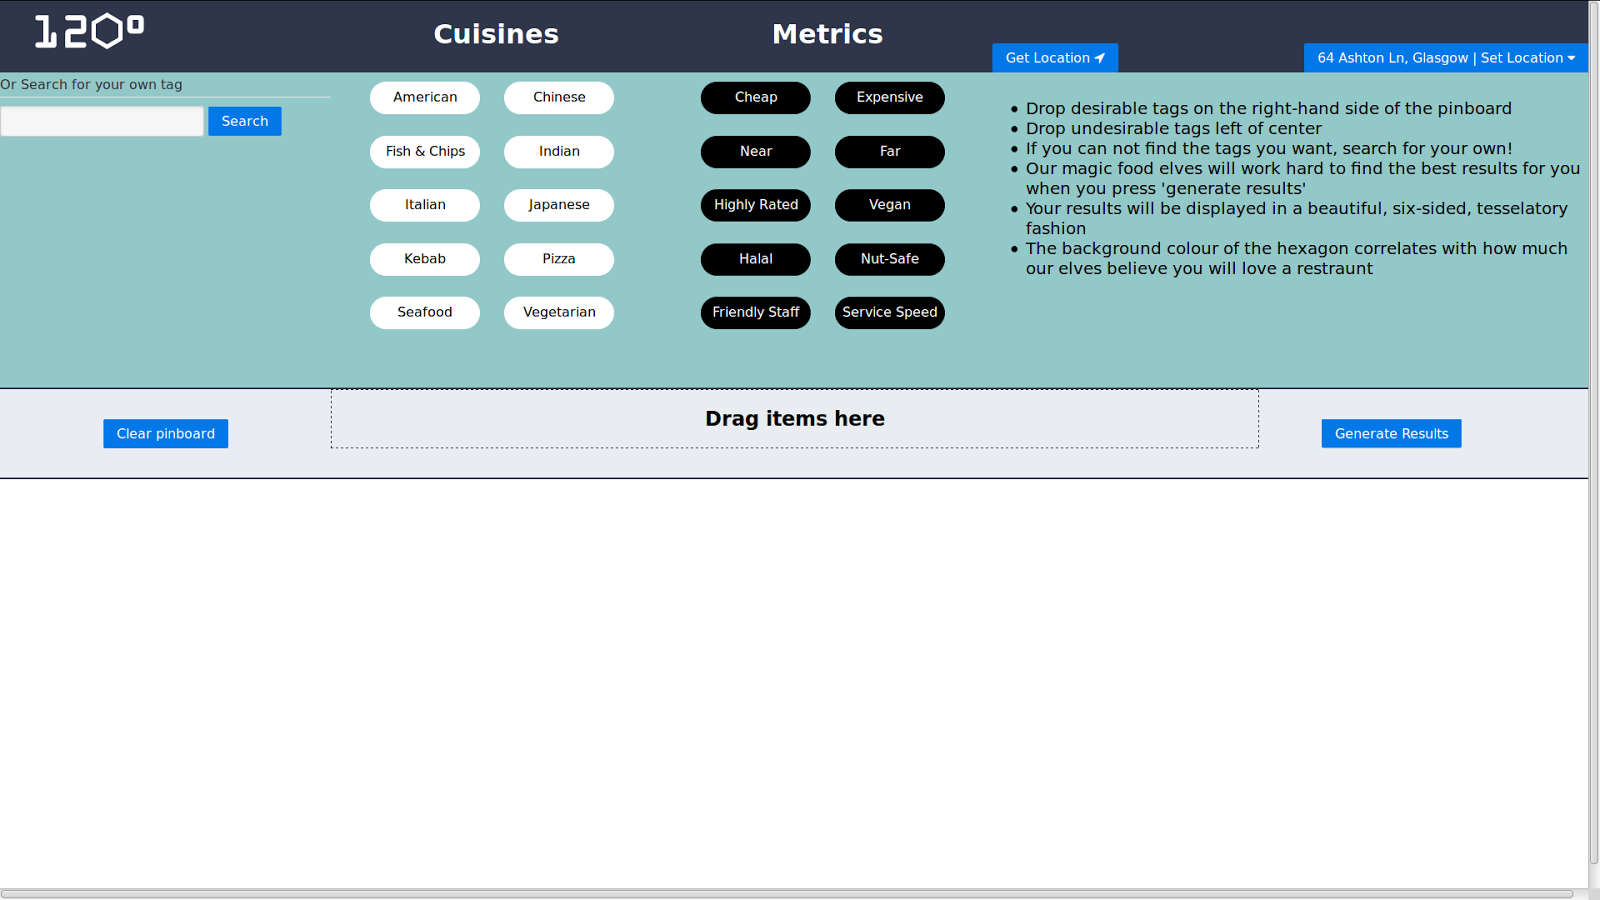
\includegraphics[scale=0.2]{oldScreenshot.png}
		\caption{Our old design before changes were made}
		\label{figure:old-design}
	\end{center}
\end{figure}

\begin{figure}[H]
	\begin{center}
		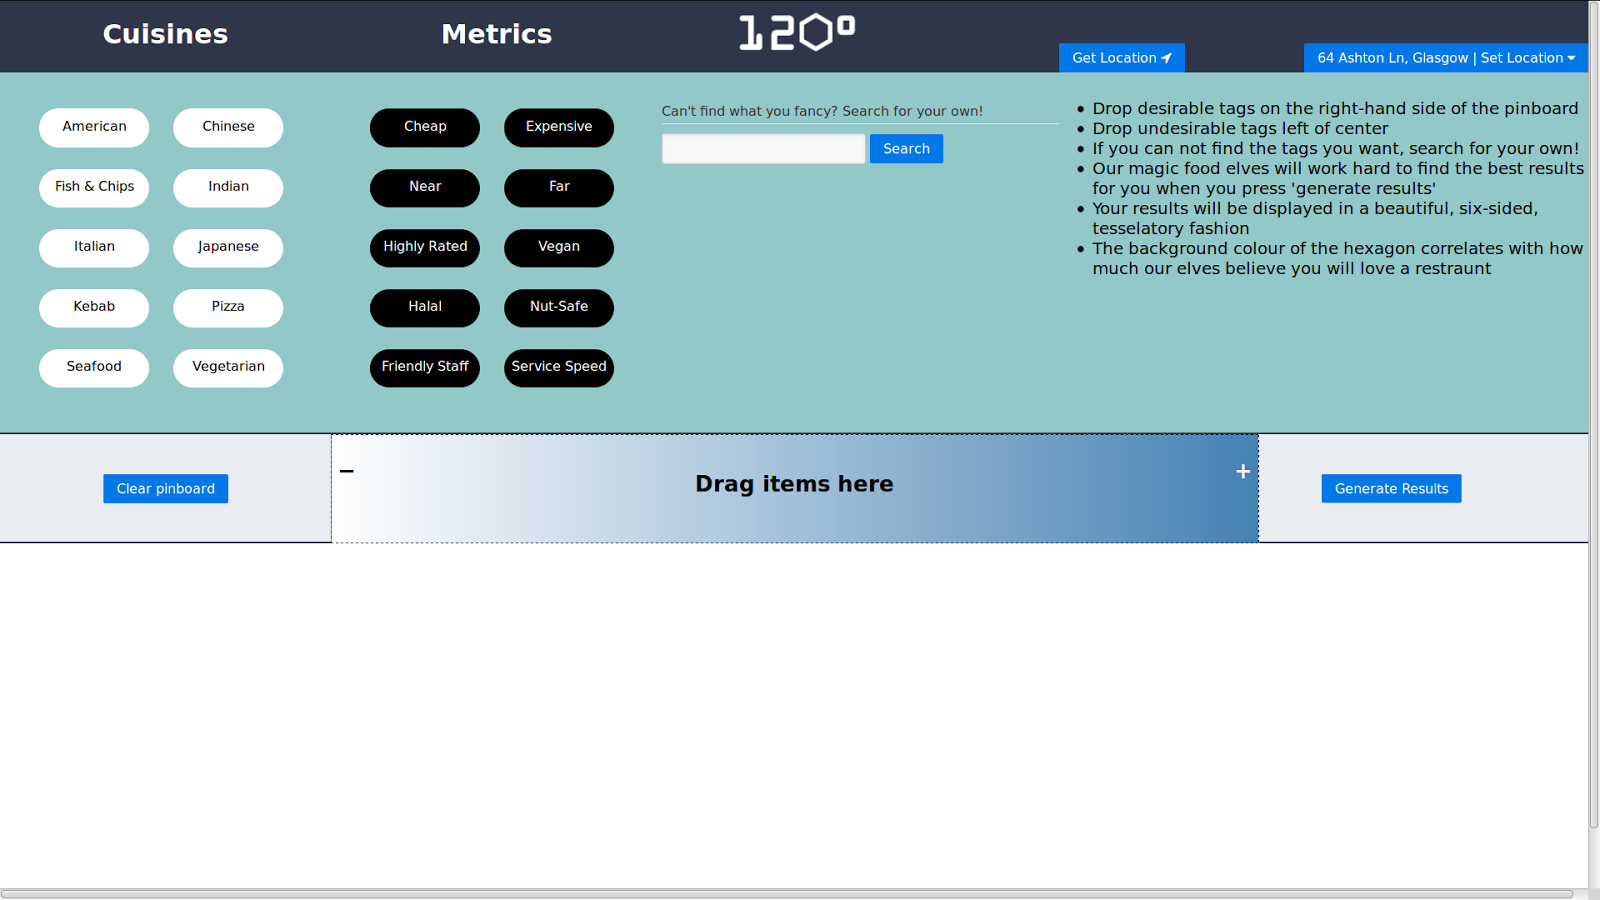
\includegraphics[scale=0.2]{superNewScreenshot.png}
		\caption{New design after changes}
		\label{figure:new-design}
	\end{center}
\end{figure}

The above are images to display the changes we made to the design of our application. 

The main item we changed was updating the pinboard, originally it had a very bland design, so much so that some of our test participants did not even notice it was there. We enlarged it, made the “drag items here” message larger, added a gradient background and ‘+’ and ‘-’ text to make the positioning of the elements of obvious. 

We rearranged all of the sections to aid with the work-flow that a user will undertake when interacting with our application, our intention was to make interaction with our application more natural. We believed it was more intuitive for users to first look at the suggestions before searching for missing items rather than the opposite, as our previous iteration had been.

We also enlarged and reworded our functionality explanation. This was an element of the design that raised much debate, it had not been in the original wireframes as we had not envisaged it as being necessary although our testing made its necessity evident. As we were limited in the amount of time we had to plan and develop the application, we were not able to implement it as effectively as perhaps we could have. Since these screenshots were taken, we have enlarged the text yet again and added more description, in particular of how the map works.


\subsection*{Experiment 2}

To ensure that our results were significant and allow for comparison between them, we gave our second group of testers the same scenarios and asked them for comments on the same sections as we did our first group. We believed that the changes we had made would lead to a reduction in the time needed for our participants to complete the tasks and that their comments would be in line with our expectation that our changes had made the system easier to use and made the work-flow transition smoother and more naturally.

\begin{itemize}

\item{User 1:

\begin{itemize}
\item{Task 1:

Time taken: 23s

User 1 was impressed by the design of the application and described it as “professional”.
User 1 was quick to pick up the system’s functionality and seemed to intuitively grasp the drag-and-drop tags and the positioning on the pinboard.
}

\item{Task 2:

Time taken: 43s

User 1 described the drag-and-drop functionality as “smooth” and said that he felt the map “worked cleanly”.
User 1’s interaction with the map was quick and precise, they were clearly comfortable with the Google Maps interface. 
}
\item{Task 3:

Time taken: 12s

User 1 had some issues with the format of the results display, although they did remark positively on the layout, they suggested we change the on-click effects of the results and prevent more than one hexagon from being expanded at a time.
}
\end{itemize}}

\item{User 2:
\begin{itemize}
\item{Task 1:

Time taken: 54s

User 2 described the gradient background of the pinboard as “word art-y”, although they liked the professional look of the banner across the top of the page.
It was clear that user 2 struggled with the dragging and was not comfortable using a touchpad rather than a mouse to perform the task, which raised issues we had not considered.
}
\item{Task 2:

Time taken: 67s

User 2 described the functionality as “fairly standard stuff for a professional web-app” although they described the dragging as “unintuitive”, though this may have been down to the input device they were using. 
As with task 1, it was clear that user 2 also had trouble with dragging the pin on the map using the trackpad.}
\item{Task 3:

Time taken: 20s

User 2 described the animation of the results as “nice” although claimed that they felt the text was too small.
It was clear that given some time to adapt, User 3 had become accustomed to using the system.
}
\end{itemize}}

\item{User 3:
\begin{itemize}
\item{Task 1:

Time taken: 10s

User 3 was fond of the colour scheme but admitted to not liking the functionality explanation, describing it as “bland”.
User 3 was clearly tech savvy, and immediately recognised the basic drag-and-drop functionality, handling it with ease.
}
\item{Task 2:

Time taken: 29s

User 3 liked the functionality and described it as “natural” although they also said they believed the map’s dragging functionality to be “not obvious”.
User 3 was comfortable with the map and had clearly used Google Maps before although they too struggled with the touchpad and dragging the small pin object.
}
\item{Task 3:

Time taken: 11s

User 3 said that the hexagons were “an interesting decision” although they were very positive about the colour scheme.
They had a very similar performance to in task one, making it clear they did not need to ‘learn’ the system as other users did.
}
\end{itemize}}

\end{itemize}


\begin{table}[H]
\centering
\begin{tabular}{c|ccc|}
\cline{2-4}
                             &                             & Time Taken (s)              &        \\ \cline{2-4} 
                             & \multicolumn{1}{c|}{User 1} & \multicolumn{1}{c|}{User 2} & User 3 \\ \hline
\multicolumn{1}{|c|}{Task 1} & \multicolumn{1}{c|}{23}       & \multicolumn{1}{c|}{44}       &  10      \\ \hline
\multicolumn{1}{|c|}{Task 2} & \multicolumn{1}{c|}{43}       & \multicolumn{1}{c|}{67}       &    29    \\ \hline
\multicolumn{1}{|c|}{Task 3} & \multicolumn{1}{c|}{12}       & \multicolumn{1}{c|}{20}       &    11    \\ \hline
\end{tabular}
\caption{Experiment 2 Results \label{table:experiment-2}}
\end{table}

\subsection*{Discussion of Findings}

In analysing the quantitative data some patterns were evident. Firstly, as we had predicted, the times taken per task decreased, as evidence best by the difference in average times, for all tasks, the testers of the earlier implementation took 46.4 seconds to complete a task where-as the participants in the test on the later implementation took 29.9 seconds, that is they were 35\% faster. However, averages of all of the tests as a single data set is not very instructive as the tests required very different inputs and therefore take varying lengths of time to complete. To remedy this, it is more significant to compare the difference in the averages per task. In tasks 1 and 2, the participants in the second test group performed better (where better is measured as faster) on average than those in the first test group, however in the final task the second group performed over 20\% slower than the first. 

\begin{figure}[H]
	\begin{center}
		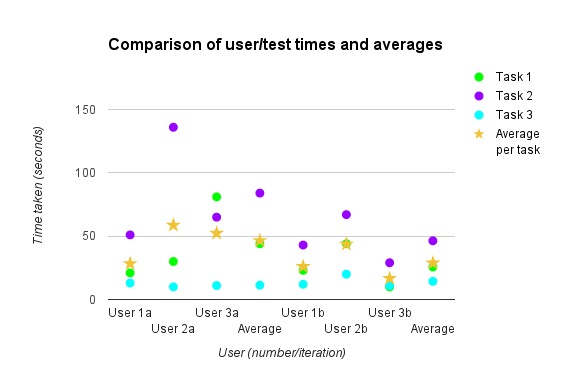
\includegraphics[scale=0.5]{graph.png}
		\caption{Graph of time taken per user and task}
		\label{figure:graph}
	\end{center}
\end{figure}

To deal with the discrepancies, it was clear that the best way to measure the result was to look for other metrics. Our tasks were designed such that tasks 1 and 3 were very similar, so similar in fact that we hypothesised that the only difference in timings was due to the time taken for participants to familiarise themselves with application’s functionality. For task 1, users had to drag three tags onto the pinboard and generate results whereas for task 3 users had to drag only two tags onto the pinboard, with one of them having to be typed into the text-field to generate it. From our results, we extracted a measurement of the time taken for participants to familiarise themselves with the system by calculating the time taken for users to complete task 1 minus the time taken for them to complete task 3. If the difference between completion of task 3 and task 1 is the time taken for users to familiarise themselves, then that difference divided by the time taken to complete task 1 will give a ratio of time taken by a participant to familiarise themselves with our system. We called this metric the ‘ratio of time to familiarise (RTTF)’ and it shows a very clear improvement when comparing test group A and B. The average RTTF of the first test group was 63.7\%, that is, given the assumptions, over half of their time was spent understanding the system rather than using it. The average RTTF of the test group for the later iteration was down to 30.8\%, that is our test participants needed less than half as much time familiarising themselves with our second iteration than they did with our first. This goes a long way to confirming our hypothesis that the changes we performed made our application more intuitive to use.

Our tests were not as accurate as they could have been owing to time constraints. The sample size was small and this will have an affect on how reliable the results we obtained will be.


\begin{table}[]

\begin{adjustbox}{max width=\textwidth}
\centering
\begin{tabular}{|p{3.5cm}!{\vrule width 2pt}r|r|r|r!{\vrule width 2pt}r|r|r|r|}
\hline
{\ul \textbf{Task}}                   & \multicolumn{1}{l|}{{\ul User 1a}} & \multicolumn{1}{l|}{{\ul User 2a}} & \multicolumn{1}{l|}{{\ul User 3a}} & \multicolumn{1}{l !{\vrule width 2pt}}{{\ul Average}} & \multicolumn{1}{l|}{{\ul User 1b}} & \multicolumn{1}{l|}{{\ul User 2b}} & \multicolumn{1}{l|}{{\ul User 3b}} & \multicolumn{1}{l|}{{\ul Average}} \\ \hline
Task 1                                & 21                                 & 30                                 & 81                                 & 44                                 & 23                                 & 44                                 & 10                                 & 25.7                        \\ \hline
Task 3                                & 13                                 & 10                                 & 11                                 & 11.3                        & 12                                 & 20                                 & 11                                 & 14.3                        \\ \hline
Time to Familiarise (Task 3 - Task 1) & 8                                  & 20                                 & 70                                 & 32.7                        & 11                                 & 24                                 & -1                                 & 11.3                        \\ \hline
\textbf{RTTF (TTF/Task 1)}            & 0.381                        & 0.667                       & 0.864                       & \textbf{0.637}              & 0.478                       & 0.545                       & -0.1                               & \textbf{0.308}              \\ \hline
\end{tabular}

\end{adjustbox}

\caption{RTTF results}
\label{rttf}

\end{table}

\section*{User Guide}

The user starts by dragging tags to either side of the pinboard. They can drag as many as they like to create their perfect search. The right half of the pinboard represents desirable tags, and the further right the tag is, the more weight the algorithm will give the tag. Tags on the left, on the other hand, are considered undesirable, and the algorithm will rank restaurants that match these tags lower than other restaurants. We have provided several suggested tags to find a specific cuisine or a good metric by which to rank the eateries. For example, a user can search for any ‘Indian’ and any ‘Chinese’ restaurants, with the metrics ‘Near’ and ‘Halal’. If the suggested tags do not encompass all the search terms the user requires, they can add their own by using the search bar and dragging their new custom tags to the pinboard. Any tags can be removed by dragging them off the pinboard. Pressing the ‘Generate Results’ button will start the algorithm, searching for the perfect restaurants and displaying the results as color-coded hexagons. The more blue the hexagon, the better it matches the search tags, and the paler, the worse it matches. Clicking on a result hexagon will change its colour and offer options to find it on a map and also a link to the restaurant’s website. Where a website is not available, an alert will appear on the screen with a phone  number allowing users an alternative method of ordering. By default, the algorithm will return results near where we think you are, but in case we are incorrect or if you are planning ahead for a meal, you can open the map and drag the pin to the desired location. Clicking the ‘Get Location’ button will make the website try to retrieve your location. 

\section*{Task Divisions}

Our team consists of six members:
\begin{itemize}
	\item Paul Cowie, 2082442c
	\item Jacob Ford, 2091723f
	\item Nicole Munro, 2081902m
	\item William Kavanagh, 2079532k
	\item Pregashni Mohanarajah, 2083114m
	\item Ben Procter, 2078440p
\end{itemize}

Paul first worked on integrating a map onto our site. Using the Google Maps API, Paul was able to create a toggleable map and incorporate a button which allowed users to find their current position using the HTML Geolocation API, given their browsers allowed location sharing. Paul then worked on the search bar functionality, generating custom tags from the search-field and ensuring searches for cuisine types were treated as such. He then created the functionality for the ‘generate results’ button, pulling associative scores from the pinboard and feeding them back into the algorithm created by Jacob for gathering suggestions. Paul also did a lot of work on the javascript and css elements on the index page to help create a professional design. He also enforced consistent code practices, separating concerns and ensuring cohesion between the several disparate elements that were created separately before all being added together in a single product.

William’s main role was to develop the front-end visuals of the site, ensuring all of the functionality of the application was wrapped in a suitable design. He provided many of the original ideas that the group expanded upon in the early design stages. William first worked on building the javascript to allow for the drag-and-drop functionality of the tags. He then created the pinboard and formed a basic algorithm in jQuery that calculates an associative score for all tags on the board. William also created the framework for the index page using pure-css to provide the grid system that divides up the page, and was responsible for ensuring the website conformed to professional styles. He did the bulk of the styling work, ensuring the CSS created an attractive but intuitive, user-friendly design. Lastly, he was responsible for generating the suggested tags and the functionality explanations on the page.

Jacob’s primary role was accessing the Google Places API, pulling large data sets for results generation, and implementing the algorithm using the user-generated results from the pinboard. Jacob was able to pull restaurant and cafe results based on proximity from the Google Places API and then process results, forming the associative scores for each eatery. In parsing the results, Jacob was able to formulate scores on a consistent range based on metric queries such as distance, price, and rating, as well as gathering results for custom user-generated tags. Jacob searched Google’s user reviews and created an algorithm to map occurrences of specific keywords to the standardised weight. Jacob also aided with the result display by working on the text positioning on the hexagons. During the final stages of the build, he provided assistance to many of the other subgroups within the team to ensure the application integrated successfully, working to quell any issues that arose from the final application’s compilation. He also worked with Paul and William to form the distinctive icon for the website.

Ben’s main role in the group was as the software architect, ensuring clarity of design in all elements of the application. Ben was responsible for maintaining a consistent design philosophy, in line with the requirements set out in the initial design phase. In his role, Ben assisted with all aspects of the final build. Ben aided in the colour-scheme, as William is colour blind, as well as helping form the full and measured wire-frame to which the system was built. Ben lended his expertise to Nicole and Pregashni in order to generate the structure of the hexagonal results display. He also worked with Paul on providing the draggable marker on the map overlay, allowing users to manually change their location on the map.

Nicole and Pregashni, from the onset of the building stage of the design worked on generating the hexagonal results display. Familiarising themselves with D3 (Data Driven Documents), their subgroup were not able to integrate their code until every other group had integrated theirs, which added another level of complexity. They formulated their own sample data and used the extensive D3 API to create hexagonal objects upon which to display a restaurant's information and allow for on-click events. Once they had created hexagonal objects, they worked on creating several at a time, this included the smooth colour gradient which denoted associative score, the tessellating design of the hexagons (for which they were helped by Ben), and the exploded view of a hexagonal object given on mouse-clicks. When their results were implemented with both Jacob’s algorithm and the scores collected by Paul, there were several integration issues which involved a large deal of reworking, which became a group effort that they led. The exploded view of the hexagon did not make the final product, but instead the colour of the hexagon changes on click.

The design of the product, the testing of it and the documentation of our results were all performed as a group. Our reports were co-written by every group member, with no text submitted that had not been reviewed by everyone. The design came from a lengthy group discussion stemming from A/B wireframe designs and pulling the best elements of everyone’s suggested designs into the coherent product that we built.


\section*{Third-Party Projects Used}

Some of the functionality of the project required the use of third-party code and REST APIs. The following list shows all external code used:

\begin{itemize}
	\item \textbf{Pure} (\url{http://purecss.io/}) was used for creating a grid layout for the index page, allowing for a fairly responsive design. It was also used for some basic page styling, such on the buttons.
	\item \textbf{Google Maps API} (\url{https://developers.google.com/maps/documentation/javascript/}) was used for creating the JavaScript map in the corner of the screen.
	\item \textbf{Google Places API} (\url{https://developers.google.com/places/javascript/}) was used for fetching results from Google based on the tag choices and positions, using our search algorithm.
	\item \textbf{jQuery} (\url{https://jquery.com/}) was used for general DOM manipulation.
	\item \textbf{Spin.js} (\url{https://fgnass.github.io/spin.js/}) was used to show a spinner while the results were loading, since the repeated requests to the Google Places API often took a significant amount of time, which initially resulted in confusion over whether or not the page was actually fetching results or not. Adding a loading spinner eliminated this problem.
	\item \textbf{Font Awesome} (\url{https://fortawesome.github.io/Font-Awesome/}) was used for icons on buttons, which helped to explain their function and state, such as the arrow on the map button which suggested that clicking it would present a dropdown.
	\item \textbf{D3} (\url{http://d3js.org/}) was used for the displaying of results, since it allows for much more interesting and dynamic visualization than plain HTML and CSS.
	\item \textbf{D3plus} (\url{http://d3plus.org/}) was used for the hexagonal display, adding to the functionality provided by D3 itself.
\end{itemize}

In addition to the software above, some snippets of code were utilized in the algorithm’s data retrieval. These are all referenced within {\tt main.js}.


\section*{Issues Faced and Conclusion}

If we had more time, the project could have been improved in certain ways. Firstly, we may have been able to improve on the design of the hexagonal display, or replace it altogether with a simpler solution. Despite this being a large focus of the project, we had a lot of problems with making the display functional and aesthetically pleasing, since the D3 library, while powerful, is somewhat difficult to use properly. We also had problems with integration, since we’d split into several subteams to work on different parts of the functionality, and had each made assumptions about the format of others’ work which was not necessarily correct.

Some of the problems that our project faced, such as a small number of results produced when ‘Generate Results’ is pressed, would not be an issue if we had access to the paid-for Google Places API, since that would remove the rate limiting. If the council were to choose this project, then they could spend a small amount on full access to the Google Places API.

Although these problems impacted on our solution, we managed to meet most of the design requirements that we set out for ourselves at the start of the project, and our testing showed that users reacted generally positively to the unique and interesting design and interaction with our system. 

\end{document}